\documentclass[a4paper,12pt]{article} % The document class with options

\usepackage[T1]{fontenc}
\usepackage{enumitem}
\usepackage{amsmath}
\usepackage{amsfonts}
\usepackage{microtype}
\usepackage{graphicx}
\usepackage{epstopdf}
\usepackage{float}
% chktex-file 1
% chktex-file 3
% chktex-file 18
% chktex-file 24
% chktex-file 25

\begin{document}
%\setlength{\parskip}{1em} 
%\setlength{\parindent}{0pt}
\newcommand{\vect}[1]{\mathbf{#1}}

\title{MECH 503 Homework 1}
\author{Jincong Li \\ 60539939}
\date{Jan 26th}
\maketitle

\section{\textbf{Question 1}}

\begin{enumerate}[label= (\alph*)]
    \item \[ \nu_i u_i = \sum_{i=1}^{n} \nu_i u_i  = \vect{v} \cdot \vect{u} \]
    
    \item \[ \delta_{ii} = \sum_{i=1}^{n} \delta_{ii} = n = 3 \]

    \item \[ \nu_{i,i} = \sum_{i=1}^{n} \frac{\partial \nu_i}{\partial x_i}  = \nabla \cdot \vect{v}\]

    \item \[ \delta_{ij,j} = \sum_{j=1}^{n} \frac{\partial \delta_{ij}}{\partial x_j} = 0\]

    \item \[ \epsilon_{ijk} v_j u_k = \sum_{j=1}^{n} \sum_{k=1}^{n} \epsilon_{ijk} v_j u_k  = \vect{v} \times  \vect{u} \]

    \item \[ \delta_{mi} \delta_{mj} T_{ij} = \sum_{i=1}^{n} \sum_{j=1}^{n} \delta_{mi} \delta_{mj} T_{ij} = T_{mm} = \text{Trace ($\vect{T}$)}\]

    \item \[ Q_{ij} T_{ik} Q_{km} = \sum_{j=1}^{n} \sum_{k=1}^{n} Q_{ij} T_{ik} Q_{km} = {\vect{Q}}^T \vect{T}\vect{Q} \]

    \item \[ \epsilon_{ijk} \sigma_{jk} = \sum_{j=1}^{n} \sum_{k=1}^{n} \epsilon_{ijk} \sigma_{jk} =0 \]
\end{enumerate}

\section{\textbf{Question 2}}

\begin{enumerate}[label= (\alph*)]
    \item \[ (u \times v) \cdot w = \varepsilon_{ijk} u_j v_k w_i \]

    \item \[ \text{det } T = \varepsilon_{ijk} T_{1i} T_{2j} T_{3k} \]
    
    \item \[ (\nabla \times v)_i = \varepsilon_{ijk} \partial_j v_k = \varepsilon_{ijk} v_{k,j}\]
    
    \item \[ \nabla \cdot v = \partial_i v_i = v_{i,i} \]
    
    \item \[ (\nabla \times T)_{ij} = \varepsilon_{jkl} \partial_k T_{il} = T_{il,k} \]
    
    \item \[ (\nabla \times (\nabla T))_i = \varepsilon_{ijk} \partial_j (\partial_k T) = T_{j,k}\]
    
    \item \[ (\nabla \cdot T)_i = \partial_j T_{ij} = T_{ij,j} \]
Since the direction of some expressions are missing, I assumed one direction when doing the index notation.
It is equavalent to add a direction vector such as $e_i$ at the end of the index notation without specifying 
a direction ahead. 
\end{enumerate}

\newpage
\section{\textbf{Question 3}}
\begin{align*}
    \intertext{Define a second order tensor $C$ such that}
    \vect{C} &= \vect{A} \cdot \vect{B}\\
    \Longleftrightarrow C_{ij} &= A_{ik} \cdot B_{kj}\\
    \text{det \textbf{C}} &= \epsilon _{ijk} C_{1i} C_{2j} C_{3k}\\
    &= \epsilon _{ijk} (A_{1l} B_{li}) (A_{2m} B_{mj}) (A_{3n} B_{nk})\\
    &= \epsilon _{ijk} (A_{1l} A_{2m} A_{3n}) (B_{li} B_{mj}  B_{nk})\\
    \intertext{Now consider the determinant of $A$ and $B$ separately}
    \text{det \textbf{A}} &= \epsilon _{lmn} A_{1l} A_{2m} A_{3n}\\
    \text{det \textbf{B}} &= \epsilon _{ijk} B_{li} B_{mj} B_{nk}\\
    \text{det \textbf{A}} \cdot \text{det \textbf{B}} &=(\epsilon _{lmn} A_{1l} A_{2m} A_{3n})(\epsilon _{ijk} B_{li} B_{mj} B_{nk})
    \intertext{Thus, one can conclude the following}
    \text{det (\textbf{A $\cdot$ B})} &= \text{det \textbf{A}} \cdot \text{det \textbf{B}}
\end{align*}

\newpage
\section{\textbf{Question 4}}
\begin{align*}
    (QQ^T)_{ij} &= Q_{ik} Q^T_{kj} \\
&= Q_{ik} Q_{jk} \\
&= \delta_{ij} \\
\implies QQ^T &= I\\
(Q^TQ)_{ij} &= Q^T_{ik} Q_{kj} \\
&= Q_{ki} Q_{kj} \\
&= \delta_{ji} \\
&= \delta_{ij} \\
\implies Q^TQ &= I \\
Q_{ij} Q^{-1}_{jk} &= Q_{ij} Q^T_{kj} = \delta_{ik} \\
    \implies Q^{-1}_{jk} &= Q^T_{kj}
\end{align*}

\newpage
\section{\textbf{Question 5}}


\begin{figure}[htbp]
    % \centering
     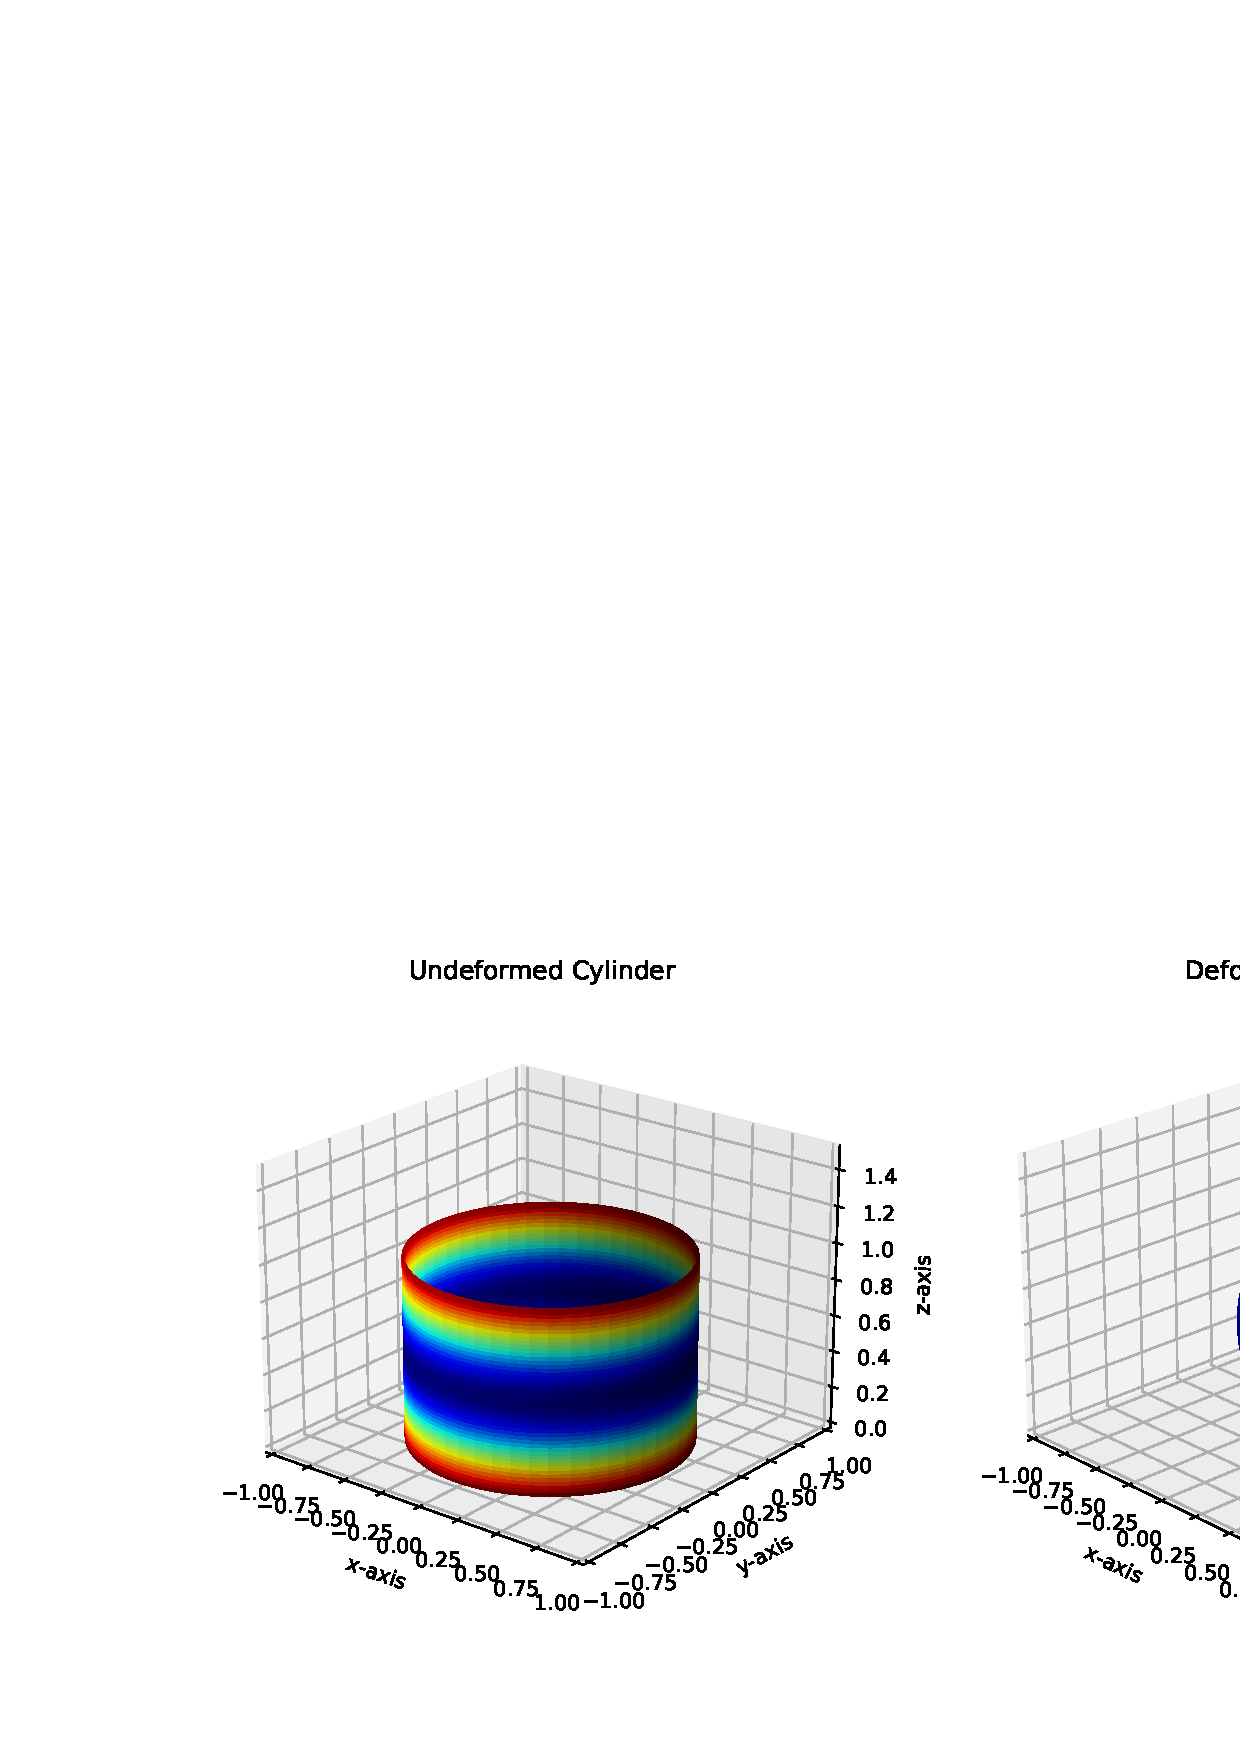
\includegraphics[scale=0.35]{MECH503HW1Q5_1.png}
    
    \caption{Undeformed and Deformed Cylinder Visualization}

\end{figure}

\subsection{Part a}
The deformation of the cylinder is characterized as follows: Viewed from above, the cylinder undergoes counterclockwise rotation, with the degree of rotation intensifying progressively with height due to the exponential term of $x_3$ in the $\phi$ function. Concurrently, the outer surface of the cylinder undergoes expansion governed by the $f$ function, where the sine term suggests maximal expansion at mid-height and minimal expansion or contraction at the extremities. The inner surface experiences a similar pattern of expansion, albeit to a lesser extent, attributable to the evaluation with smaller inner radii $r$.
The visualization of this deformation is provided in the figure 1 above.

\subsection{Part b \& c}
The deformation as well as the Lagrangian and Eulerian strain tensors are computed in MATLAB and they are both plotted in figure 1 above.
Notice that the Lagrangian strain tensors are plotted as coloring the undeformed cylinder due to its nature of referring the undeformed configuration.
And the Eulerian strain tensors are plotted as coloring the deformed cylinder since it refers to the deformed configuration.

\subsection{Part d}
\begin{figure}[H]
    % \centering
    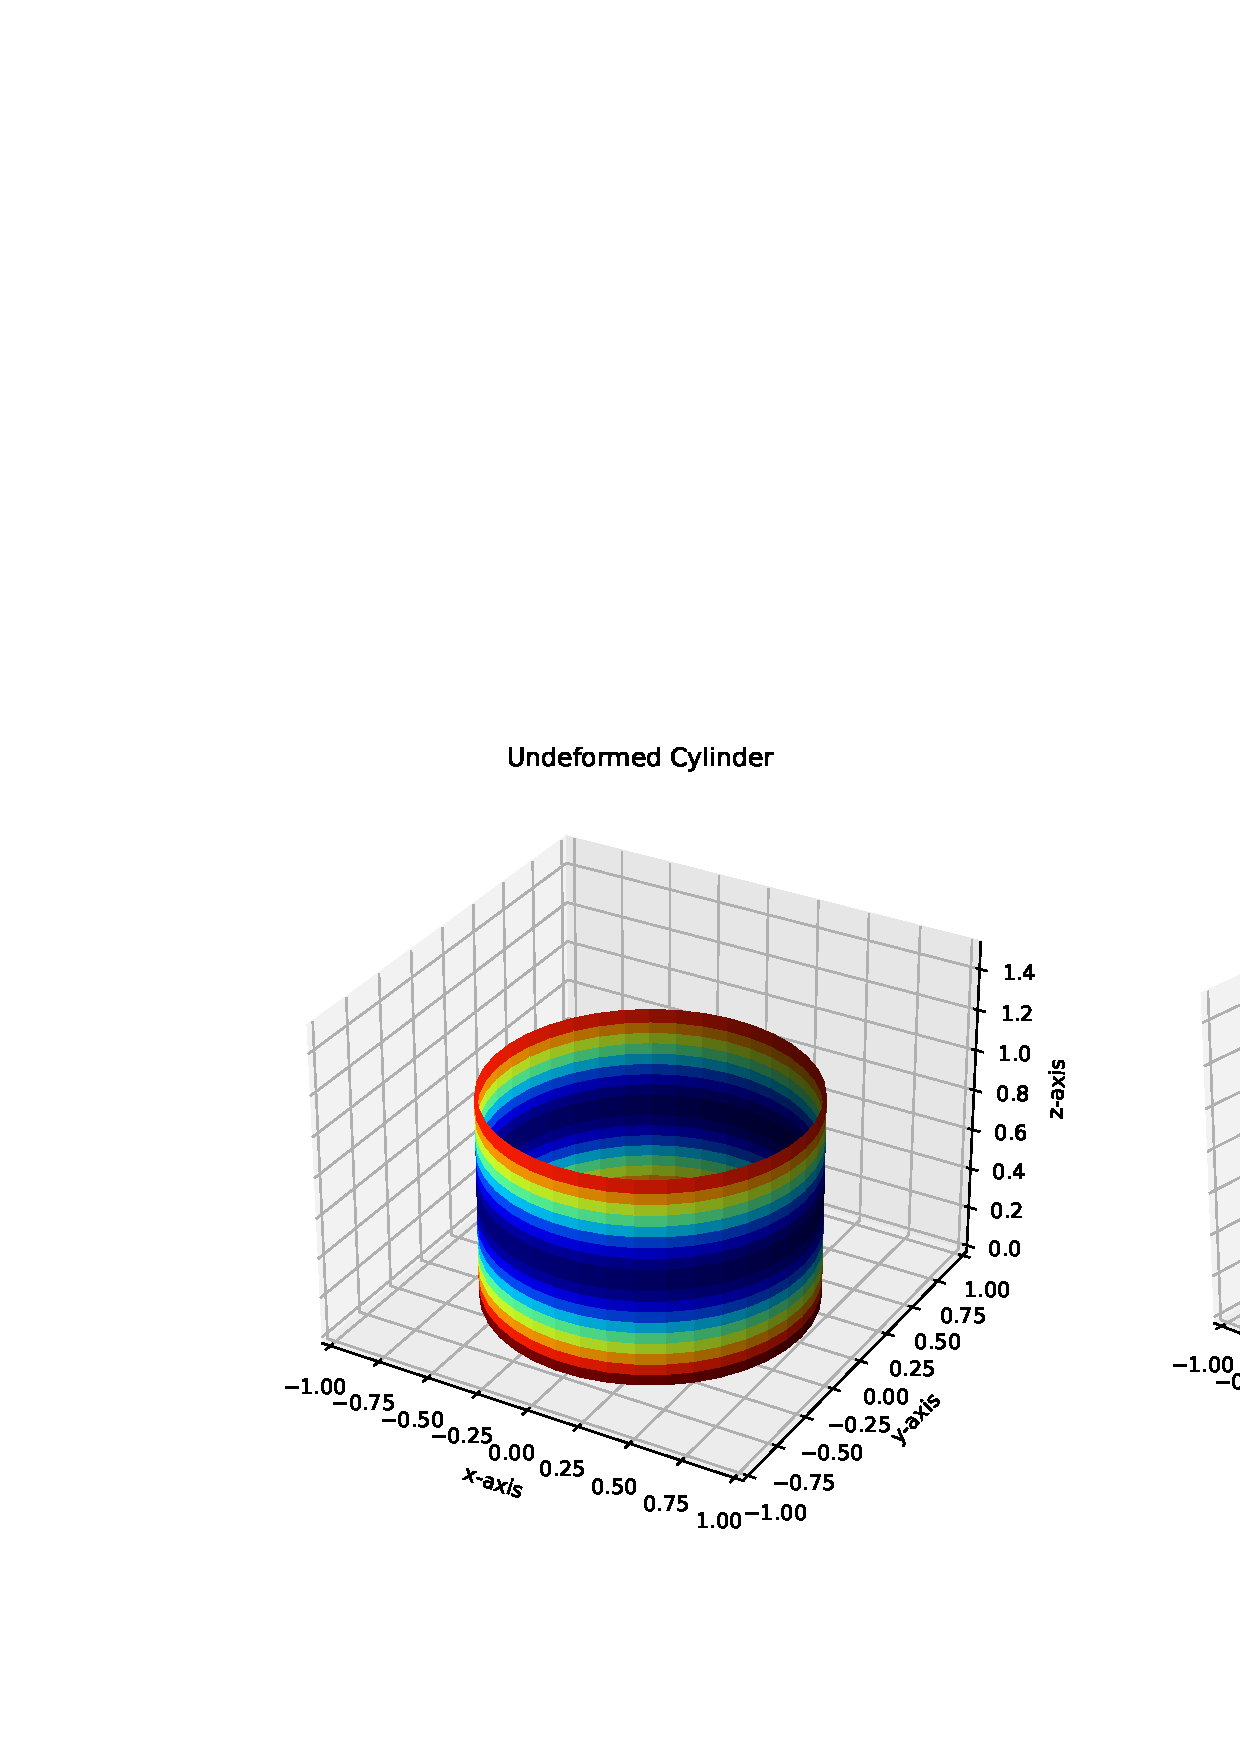
\includegraphics[scale=0.7]{MECH503HW1Q5_2.png}
    \caption{Change of length for points along vector $[1,1,0]$ on inner surface}
     
    \includegraphics[scale=0.7]{MECH503HW1Q5_3.png}
    \caption{Change of length for points along vector $[1,1,0]$ on outter surface}


\end{figure} 
Figure 2 shows the change of length for each point along the vertical axis in the direction of vector $[1,1,0]$ on outter surface.
The y-axis is the magnitude of change of length, and the x-axis is the index of point along the vertical axis in the direction of vector $[1,1,0]$.
The result makes sense since the deformation follows a sin function as discussed. Similarity could be observed on the inner surface.
Figure 3 shows the change of length for each point along the vertical axis in the direction of vector $[1,1,0]$ on inner surface.

\subsection{Part e}
\begin{figure}[H]
    % \centering
    \includegraphics[scale=0.7]{MECH503HW1Q5_4.png}
    \caption{Change of angle between $[1,1,0]$ and $[0,1,1]$ on the inner surface}
     
    \includegraphics[scale=0.7]{MECH503HW1Q5_5.png}
    \caption{Change of angle between $[1,1,0]$ and $[0,1,1]$ on the outter surface}
\label{figure2}
\end{figure}
Figure 4 presents the change of angle between $[1,1,0]$ and $[0,1,1]$ on the inner surface. Notice the values on the y axis on the plot 
represents the change of angle with respect to the previous\slash lower point (smaller index means lower height in vertical direction). This explains
why the change of angle is not exponential to the height. We know that accoring to the exponential term in $\phi$ function, any arbitrary angle should grow 
exponentially, however, these plots are not showing in that way. 
Figure 5 presents the change of angle between $[1,1,0]$ and $[0,1,1]$ on the outter surface.
     
\end{document}